\documentclass[a4paper]{scrreprt}

%%% PACKAGES %%%

% add unicode support and use german as language
\usepackage[utf8]{inputenc}
\usepackage[ngerman]{babel}

% Use Helvetica as font
\usepackage[scaled]{helvet}
\renewcommand\familydefault{\sfdefault}
\usepackage[T1]{fontenc}

% Better tables
\usepackage{tabularx}

% Better enumerisation env
\usepackage{enumitem}

% Use graphics
\usepackage{graphicx}

% Have custom abstract heading
\usepackage{abstract}

% Need a list of equation
\usepackage{tocloft}
\usepackage{ragged2e}

% Better equation environment
\usepackage{amsmath}

% Symbols for most SI units
\usepackage{siunitx}

% Bibliography & citing
\usepackage[
	backend=biber,
	style=apa,
	bibstyle=apa,
	citestyle=apa,
	sortlocale=de_DE
	]{biblatex}
\addbibresource{Referenzen.bib}

%%% COMMAND REBINDINGS %%%
\newcommand{\tabitem}{~~\llap{\textbullet}~~}

% Define list of equations - Thanks to Charles Clayton: https://tex.stackexchange.com/a/354096
\newcommand{\listequationsname}{\huge{Formelverzeichnis}}
\newlistof{myequations}{equ}{\listequationsname}
\newcommand{\myequations}[1]{
	\addcontentsline{equ}{myequations}{\protect\numberline{\theequation}#1}
}
\setlength{\cftmyequationsnumwidth}{2.3em}
\setlength{\cftmyequationsindent}{1.5em}

% Usage {equation}{caption}{label}
\newcommand{\indexequation}[3]{
	\begin{align} \label{#3} \ensuremath{\boxed{#1}} \end{align}
	\myequations{#3} \centering \small \textit{#2} \normalsize \justify }

%%% PATH DEFINITIONS %%%
% Define the path were images are found
\graphicspath{{./img/}{./pdf/}}

%%% TITLEPAGE %%%

\title{Projektdokumentation}
\subtitle{PAWI HS18}
\author{Pascal Baumann, Dane Wicki}
\publishers{Richard Wetzel}
\date{\today}

%%% DOCUMENT %%%

\begin{document}

\begin{titlepage}
\maketitle
\end{titlepage}

\renewcommand{\abstractname}{Management Summary}
\begin{abstract}
	Hier könnte ihr Management Summary stehen.
\end{abstract}

\section*{Versionskontrolle}

\begin{tabularx}{\textwidth}{|c|c|c|X|}
	\hline
	\textbf{Versionsnummer} & \textbf{Kürzel} & \textbf{Datum} & \textbf{Beschreibung} \\
	\hline
	0.1 & PB & 10.09.18 & Erste Versionierung \\
	\hline
\end{tabularx}

\tableofcontents

\chapter{Einführung}

\chapter{Problemstellung und Vision}

\chapter{Stand der Forschung}

\section{Technologische Grundlagen}
Als Augmented Reality (dt. erweiterte Realität) versteht man heutzutage meistens das Vermitteln von Zusatzinformationen über die Umgebung in Form von Animationen, Einblendungen und Tonwiedergaben. In den meisten Fällen wird dies über Smartphones oder Computer bewerkstelligt, es existieren jedoch auch spezialisierte Geräte wie die Microsoft HoloLens oder Google Glass. Der Term wurde erstmals von \citeauthor{Milgram1994} im Jahre 1994 detailliert definiert, wobei sie die Vermischung der realen und virtuellen Welt betrachten und worin die Technologie Augmented Reality fällt (siehe \ref{fig:RVContiinum}):

\vspace{1em}

\textquotedblleft the above-mentioned broad definition of Augmented Reality –  \textquoteleft augmenting natural feedback to the operator with simulated cues\textquoteright\ – is quite clear. Also noteworthy in this figure is the corresponding concept of Augmented Virtuality (AV), which results automatically, both conceptually and lexically, from the figure. \textquotedblright\ \parencite{Milgram1994}

\begin{figure}[htb]
	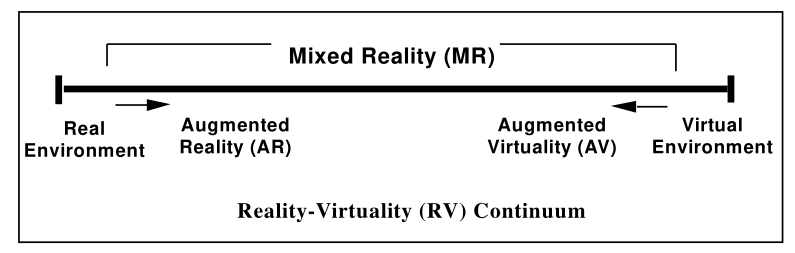
\includegraphics[keepaspectratio, width=\textwidth]{MR_milgram.png}
	\caption{Simplified representation of a RV continuum \parencite{Milgram1994}}
	\label{fig:RVContiinum}
\end{figure}



Fünf Jahre nach Milgram veröffentlichten \citeauthor{Kato1999} ihre Ergebnisse zu einem Marker-basierten AR Konferenzsystem. Sie lösten dabei das Problem der Registrierung (wo befindet sich der Benutzer, oder besser gesagt dessen Augen), und das Ermitteln der Pose (wie ist die Orientierung der virtuellen Kamera in Bezug zur Umwelt) über Marker mit einer fixen Grösse \parencite{Kato1999}. Das System war stationär mit Computern realisiert. In den folgenden Jahren wurden Versuche mit  mobilen Prototypen durchgeführt, dies blieben jedoch in der Grösse von Rucksäcken und gebrauchten Notebooks mit der entsprechenden Rechenleistung.

Ein grosser Durchbruch wurde deshalb von \citeauthor{Klein2009} erbracht, welche einen PTAM (Parallel Tracking and Mapping) Algorithmus auf einem iPhone 3G implementierten. Dieser war in der Lage sowohl in Räumen wie ausserhalb von Gebäuden, nach einer Initialisierungsphase die Lokalisierung von einem Marker loszulösen und die Pose der Kamera über \textquotedblleft Key Features\textquotedblright\ zu ermitteln \parencite{Klein2009}. Seither wurde auf diesem Gebiet weiter entwickelt und Algorithmen dieser Art sind unter dem Namen SLAM (Simultaneous Location and Mapping) zusammengefasst, dazu existieren verschiedene Frameworks welche diese nativ mitbringen (Kudan, wikitude).

\section{Anwendungen}

Auch im Bereich des BIM (Building Information Modelling) wurde im Zuge der Fortschritte in AR verschieden Lösungen erarbeitet. Neben spezialisierten Fachlösungen wie beispielsweise die DAQRI Smart Glasses (welche für AR und BIM im Industrieumfeld eingesetzt werden) \parencite{DAQRI2018}, wurde auch im wissenschaftlichen Umfeld interessante Prototypen entwickelt. So beispielsweise das Auto AR \parencite{Opperman2015} welche einem Benutzer erlaubt Neu- und geplante Bauten aus einem Auto zu begutachten, oder eine selbstentwickeltes BIM Framework des Frauenhofer Institut in Darmstadt \parencite{Olbrich2013}. Dennoch sind die Systeme von spezialisierter Hardware (GPS Sensoren, Serverbackend für Berechnungen) abhängig. Das Ziel unserer Arbeit soll sein BIM mittels einer AR Lösung auf handelsübliche Geräte (Smartphones, Tablets) zu bringen.

\chapter{Ideen und Konzepte}

\chapter{Methode}

\section{Vorgehensmodell}
% Beschreibung der agilen Projektmethode

\section{Anforderungsanalyse}

\section{Systemarchitektur}

\section{Komponentendesign}

\section{Umsetzung Programmierung}

\section{Testing}

\subsection{Testplan}

\subsection{Testfälle}

\chapter{Realisierung}

% TODO Ein Beispiel für den Gebrauch von Formeln und Referenz auf die jeweilige Formel - entfernen wenn nicht mehr gebraucht
Die Distanz zwischen zwei Geopositionen wird über die Bogenlänge (siehe \ref{Bogenlaenge}) der Differenz der Längen- und Breitengrade ausgerechnet.

\indexequation{b = \frac{\pi}{\SI{180}{\degree}}\beta r}{Bogenlänge des Winkels $\beta$ mit Radius $r$}{Bogenlaenge}

\section{Einschränkungen und Abgrenzungen}

\section{Projektmanagementplan}

\subsection{Projektorganisation}
Da beide Projektmitglieder ihre Kompetenzen eher in den technischen Bereichen dieses Projekts sehen, wurde von einer strikten Aufgabenteilung abgesehen.

Es wurde dennoch darauf geachtet, dass beide Mitglieder klare Verantwortungen übernehmen. Diese waren jedoch mehr in einer überwachenden Funktion gesehen, und soll nicht heissen, dass dieses Mitglied die Arbeit alleine leistete.

\vspace{1em}

\begin{tabularx}{\textwidth}{|X|X|}
	\hline
	\textbf{Teammitglied} & \textbf{Funktionen} \\
	\hline
	Pascal Baumann & \tabitem Dokumentation \\
	& \tabitem Testplanung \& Durchführung \\
	& \tabitem Projektmanagement \\
	\hline
	Dane Wicki & \tabitem Architektur \\
	& \tabitem Plattformanalyse \\
	\hline
\end{tabularx}

\subsection{Projektführung}

\subsection{Rahmenplan}

Das Projekt wurde in 6 zweiwöchige Sprints unterteilt und in diesen iterativ entwickelt.

\vspace{1em}

\begin{figure}
	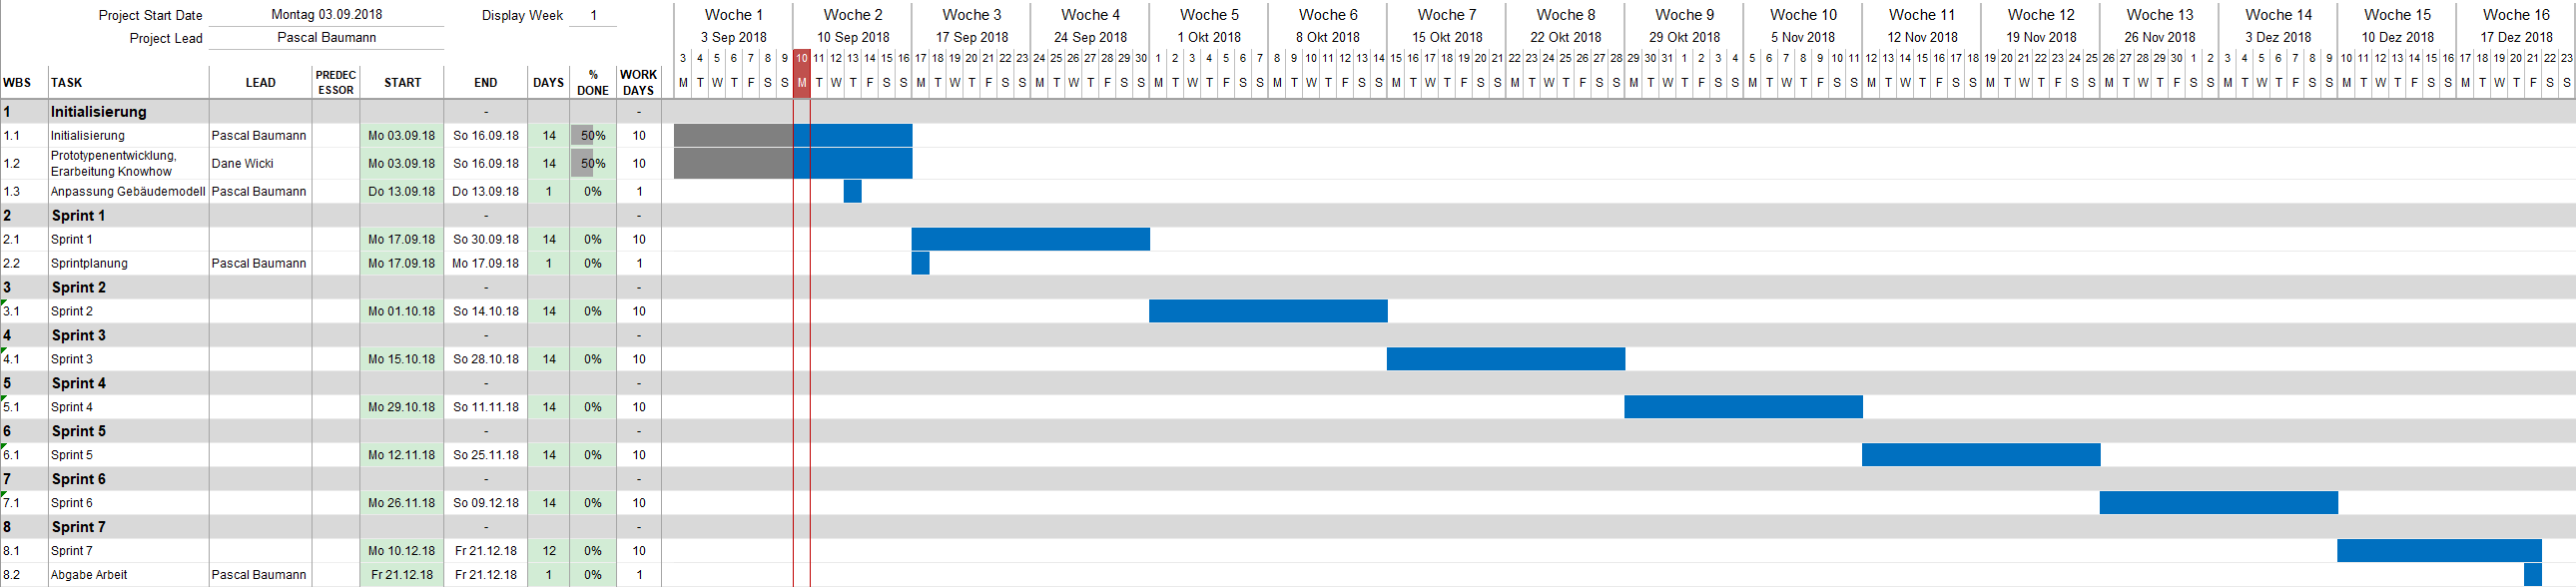
\includegraphics[keepaspectratio, width=\textwidth]{Rahmenplan}
	\caption{Überblick der Sprints}
\end{figure}

\section{Systemspezifikation}

\subsection{Systemübersicht}

\subsection{Architektur \& Design}

\subsection{Schnittstellen}

\subsection{Anforderungen}

\subsection{Anwendung}

\chapter{Evaluation und Validation}

\chapter{Ausblick}

\appendix

\chapter{Testprotokolle}


\glossary{Abkürzungsverzeichnis}

\listoffigures

\listoftables

\listofmyequations \pagebreak

\printbibliography

\chapter*{Eidesstattliche Erklärung}
Ich erkläre hiermit, dass ich/wir die vorliegende Arbeit selbständig und ohne unerlaubte fremde Hilfe angefertigt haben, alle verwendeten Quellen, Literatur und andere Hilfsmittel angegeben haben, wörtlich oder inhaltlich entnommene Stellen als solche kenntlich gemacht haben, das Vertraulichkeitsinteresse des Auftraggebers wahren und die Urheberrechtsbestimmungen der Fachhochschule Zentralschweiz (siehe Merkblatt «Studentische Arbeiten» auf MyCampus) respektieren werden.

\vspace{1em}

\renewcommand{\arraystretch}{2}
\begin{tabularx}{\textwidth}{XXXX}
	Unterschrift: & & Unterschrift: & \\ \cline{2-2}\cline{4-4}
	Baumann, Pascal & & Wicki, Dane & \\
	Datum: & & Ort: & \\
\end{tabularx}

\end{document}